\clearpage
\appendix
\section{Appendix}

\subsection{Dataset}
\label{appendix:dataset}
% \textbf{CNNDailyMail}
% \textbf{ShareGPT}
% \textbf{InstructCoder}
% \textbf{GSM8K}
% \textbf{AIME22-24}
% \textbf{GPQA-Main}
\begin{figure}[h]
    \centering
    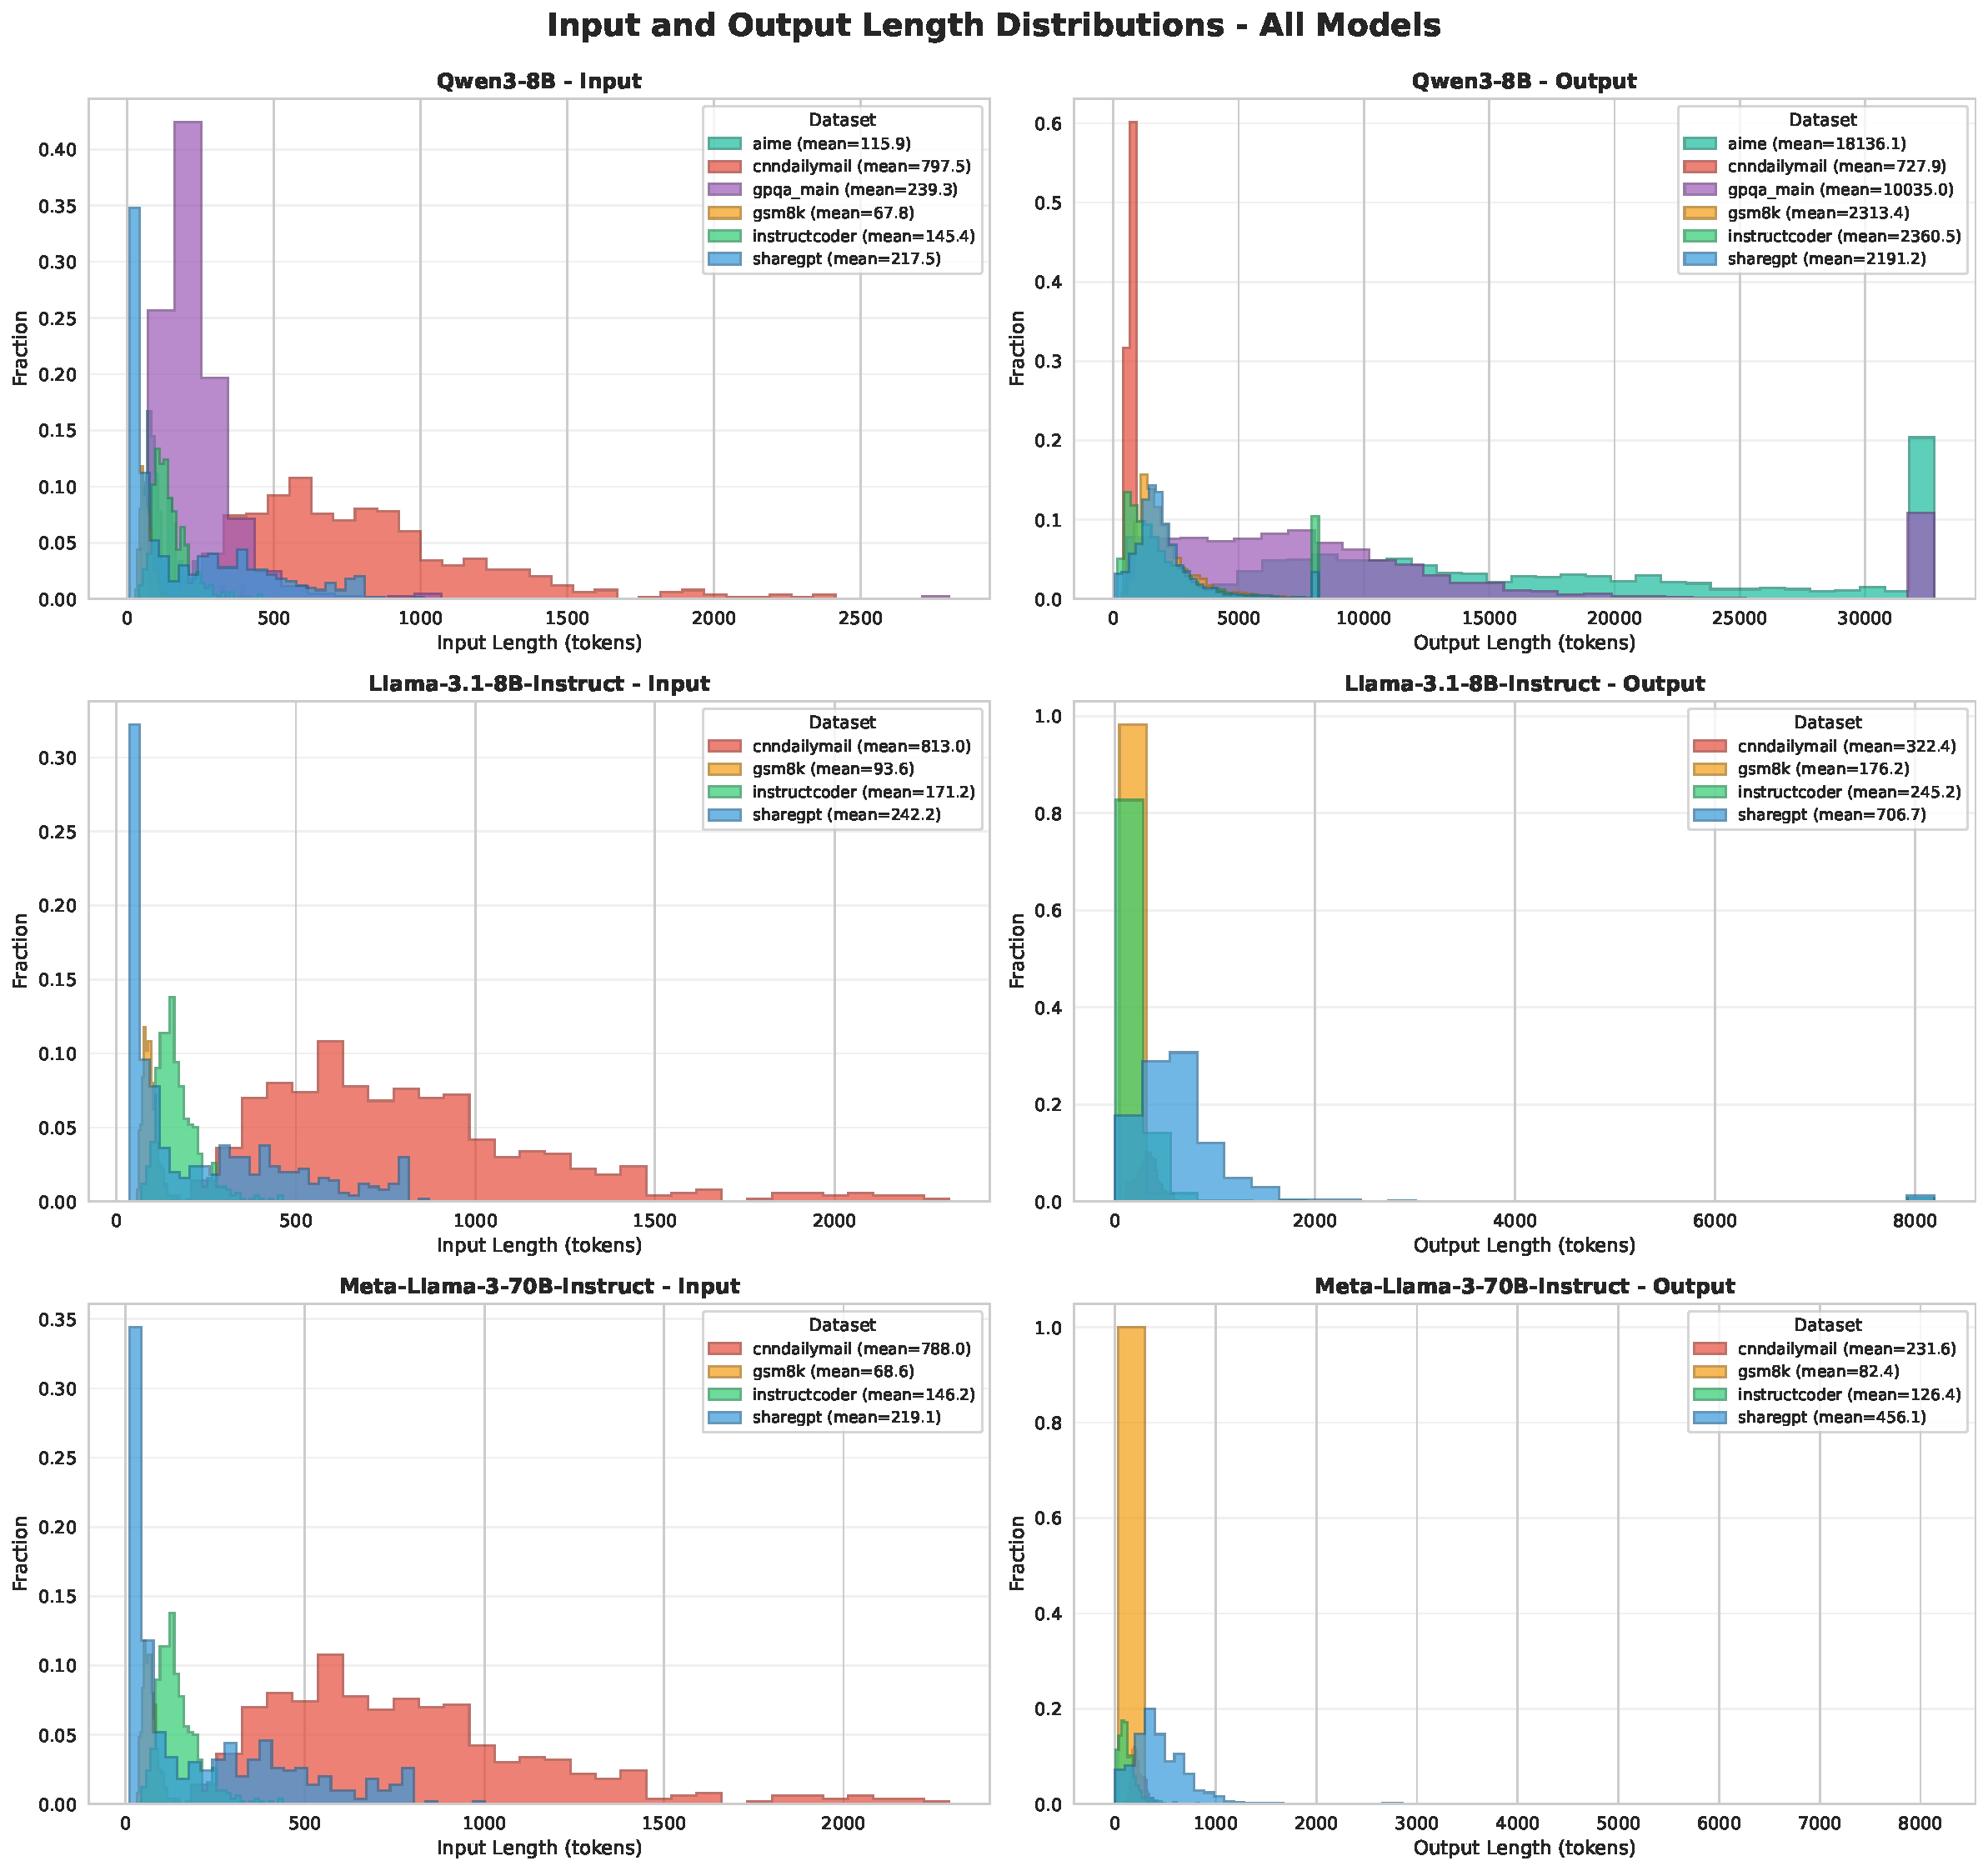
\includegraphics[width=\linewidth]{figures/workload_length_distribution/before_filtering/all_models_combined.pdf}
    \caption{Dataset Input/Output Length distributions.}
    \label{fig:dataset-input-output-plot}
\end{figure}

\subsection{Memory Breakdown Calculations}
\label{appendix:mem}
\paragraph{Static memory (GiB).} Assuming FP16 weights (2 bytes/param), the static GPU memory for model weights:
\[
M_\text{static,GiB}=\frac{(P_\text{target}+P_\text{draft})\cdot 2}{2^{30}}
\]
Here, $P_\text{target}$ is the target model's parameter size and $P_\text{draft}$ includes any additional parameters introduced by the speculative decoding method, both in units of Billions.

For EAGLE/EAGLE3, $P_\text{draft}$ refers to the parameters used in speculative decoding. For the EAGLE models we used, $P_\text{draft}$ refers to the parameter size of the autoregressive head, which includes one decoding layer and one fully connected (FC) layer. They share the same embedding layer and language modeling (LM) head with the target model. For the EAGLE3 models we used, $P_\text{draft}$ refers to the parameter size of the entire EAGLE3 model. It includes one decoding layer, the multi-layer feature fusion FC layer, a final normalization layer and its own LM head. In addition, the model checkpoints include two 1-dimensional token-id remapping tables (\texttt{t2d} and \texttt{d2t}) that translate between the target model’s vocabulary and the draft LM head’s vocabulary; they typically contribute negligibly to the parameter memory. When loading model weights in vLLM v0.10.1.1, the \texttt{t2d} tensors are skipped, and we exclude them when counting the parameter size. Similarly, these EAGLE3 models reuse the same embedding layer from the target models.

For Qwen3-0.6B, \textit{tie\_word\_embeddings} defaults to True and its LM head shares the same weight matrix as the embedding layer; thus, we exclude the size of its language modeling (LM) head.

For example, the static memory for Llama3-70B-Instruct with Llama3.2-1B-Instruct as the draft model is $(70.55+1.23)*10^9*2/2^{30}=~133.7GiB$. For Llama3.1-8B-Instruct with EAGLE-LLaMA3.1-Instruct-8B, it is $(8.03+0.25)*10^9*2/2^{30}=15.42GiB$.

\paragraph{Per-token KV cache (KiB).}
To calculate the KV cache size of each generated token:
\[
M_\text{KV/token,KiB}=
\frac{L_\text{h}\cdot 2 \cdot n_\text{kv}\cdot d_\text{head}\cdot 2}{2^{10}} .
\]
$L_\text{h}$ is the number of hidden layers,
$n_\text{kv}$ is the number of KV heads (since our models are all Grouped-Query-Attention-based),
$d_\text{head}$ is the head dimension, the first factor $2$ is for both Key and Value, and the last factor $2$ is bytes/element for FP16. For Llama3-70B-Instruct without speculative decoding or model-free SD methods like $n$-gram, it is $80*2*8*128*2/2^{10}=~320KiB$. Similarly, for Llama3.1-8B-Instruct, it is $32*2*8*128*2/2^{10}=~128KiB$.

For draft-model-based SD, the total per-token KV cache is the sum over each generated token by the target and draft model. For Llama3-70B-Instruct with Llama3.2-1B-Instruct as the draft model, the per-token KV cache memory size is $80*2*8*128*2/2^{10}$ + $16*2*8*64*2/2^{10}$ = $352KiB$.

Similarly, for EAGLE-based SD, the total per-token KV cache is the sum over each generated token by the target and EAGLE heads. For Llama3-70B-Instruct with Llama3.2-1B-Instruct as the draft model, the per-token KV cache memory size is $80*2*8*128*2/2^{10}$ + $1*2*8*128*2/2^{10}$ = $324KiB$. The value 1 here means that EAGLE uses an additional transformer block for proposal generation, which effectively adds one extra layer.

\begin{table}[t]
\centering
\small
\setlength{\tabcolsep}{4pt}
\begin{tabular}{l|rrrr}
\toprule
Model & $P$ & $L$ & $n_\text{kv}$ & $d_\text{head}$ \\
\midrule
Llama3.1-8B-Instruct  & 8.03B & 32 & 8 & 128 \\
Llama3-70B-Instruct   & 70.55B & 80 & 8 & 128 \\
Llama3.2-1B-Instruct  & 1.23B & 16 & 8 & 64 \\
Qwen3-8B              & 8.19B & 36 & 8 & 128 \\
Qwen3-0.6B              & 0.596B & 28 & 8 & 128 \\
EAGLE-LLaMA3.1-Instruct-8B & 0.25B & 1 & 8 & 128 \\
EAGLE3-LLaMA3.1-Instruct-8B & 0.425B & 1 & 8 & 128 \\
EAGLE-LLaMA3-Instruct-70B & 0.99B & 1 & 8 & 128 \\
EAGLE3-Qwen3-8B            &  0.40B     & 1 & 8 & 128 \\
\bottomrule
\end{tabular}
\vspace{2pt}
\caption{Model specs used for memory calculations. $P$ is the parameter size of the weights used, obtained by counting their parameters; $L$ is the number of hidden layers, $n_\text{kv}$ is the number of Key/Value heads, and $d_\text{head}$ is the head dimension, obtained from the model's configuration files on Hugging Face.}
\label{tab:mem_model_specs}
\vspace{-0.10in}
\end{table}


\subsection{Acceptance Behaviour}
\label{appendix:acc-behaviour}

% \begin{figure}[h!]
%   \centering
%  \begin{subfigure}{0.45\linewidth}
%     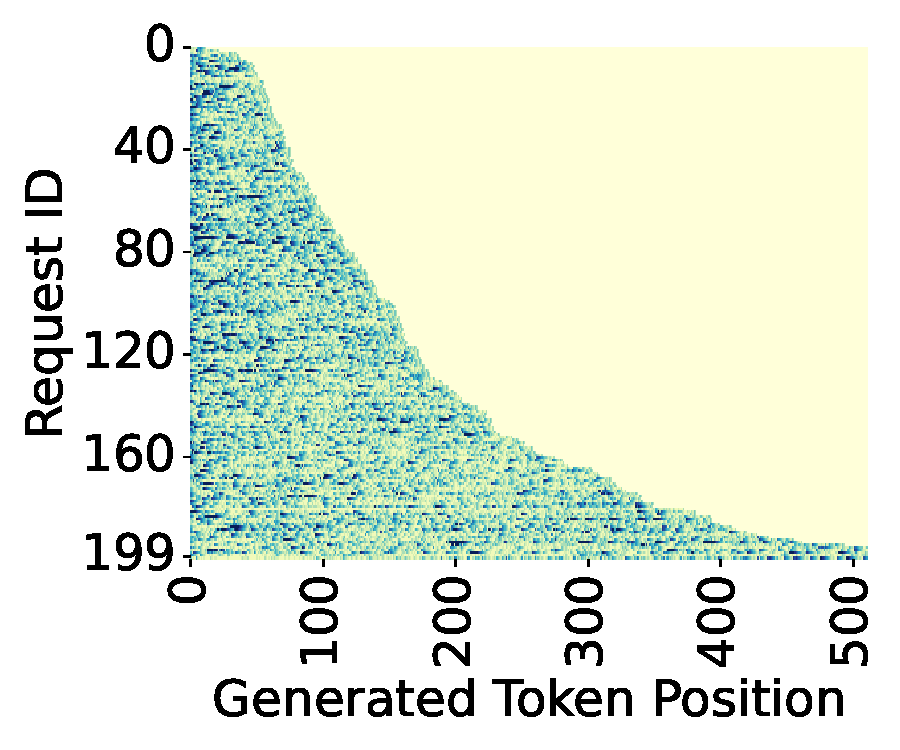
\includegraphics[width=\linewidth]{figures/acc_len/heatmap/instructcoder_eagle_llama3.1-8B_acceptance_stats.pdf}
%     \caption{InstructCoder, EAGLE}
%   \end{subfigure}
%   \hspace{1pt}
%   \begin{subfigure}{0.45\linewidth}
%     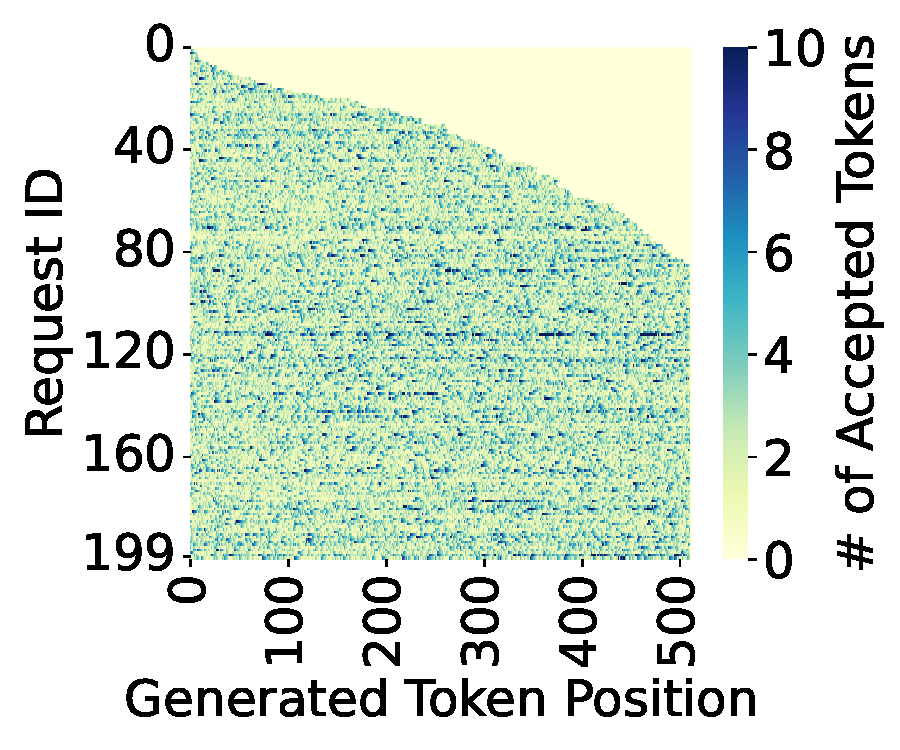
\includegraphics[width=\linewidth]{figures/acc_len/heatmap/sharegpt_eagle_llama3.1-8B_acceptance_stats.pdf}
%     \caption{ShareGPT, EAGLE}
%   \end{subfigure}
%   \caption{Generated length per token position for Llama3.1-8B. Requests are sorted based on generation length.}
%   \label{fig:acceptance-length-heatmap-continued}
% \end{figure}

% \begin{figure} [h!]
% \captionsetup{justification=centering}
%   \centering
%     \hspace{1pt}
%     \begin{subfigure}{0.45\linewidth}
%     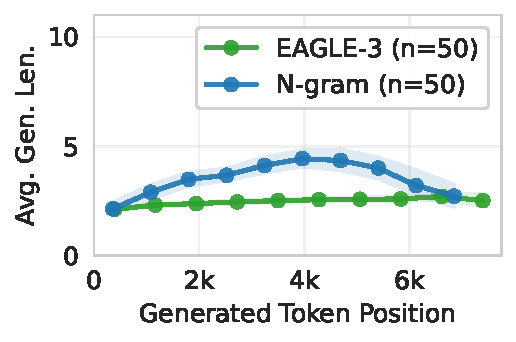
\includegraphics[width=\linewidth]{figures/acc_len/token_level/overlaid_binned_positions_gpqa_main_Qwen3-8B_bin1_range4190-7811.pdf}
%     \caption{Requests with outputs of 4K-8K tokens}
%   \end{subfigure}
%     \hspace{1pt}
%     \begin{subfigure}{0.45\linewidth}
%     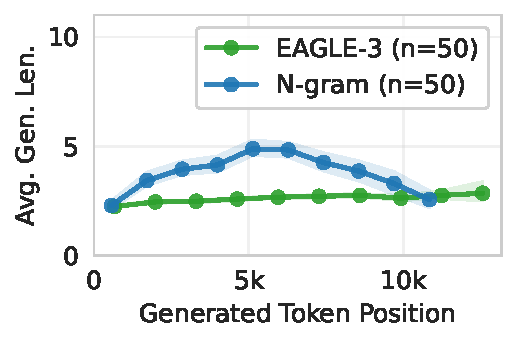
\includegraphics[width=\linewidth]{figures/acc_len/token_level/overlaid_binned_positions_gpqa_main_Qwen3-8B_bin2_range7811-13351.pdf}
%     \caption{Requests with outputs of 8K-13K tokens}
%   \end{subfigure}
% \caption{Token-level: Average generated token length per generated token position for Qwen3-8B-Thinking on GPQA-Main.}
%   \label{fig:acc-len-token-level-continued}
% \end{figure}

\begin{figure}[h]
  \centering
  
\includegraphics[width=0.7\linewidth]{figures/acc_len/request_level/legend.pdf}
  
    \begin{subfigure}{0.3\linewidth}
    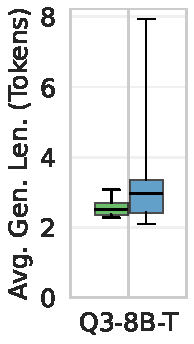
\includegraphics[width=\linewidth]{figures/acc_len/request_level/box_by_model_aime_acc_len.pdf}
    \caption{AIME22-24}
  \end{subfigure}
      \hspace{5pt}
    \begin{subfigure}{0.3\linewidth}
    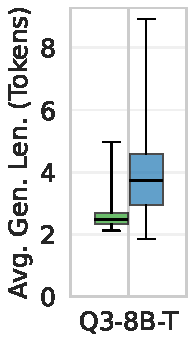
\includegraphics[width=\linewidth]{figures/acc_len/request_level//box_by_model_gpqa_main_acc_len.pdf}
    \caption{GPQA-Main}
  \end{subfigure}
\caption{Request-level generated length across datasets and models. Each box shows the distribution of per-request mean accepted length, with the box spanning the 25th–75th percentiles and whiskers covering the 5th–95th percentiles. Model used is Qwen3-8B-Thinking.}
  \label{fig:acc-len-request-level-box-plot-reasoning}
\end{figure}

\begin{table}[h!]
\centering
\begin{tabular}{llccc}
\toprule
Dataset & Method & Mean & Median & Std \\
\midrule
InstructCoder & $n$-gram & 7.27 & 6.57 & 4.19 \\
InstructCoder & EAGLE & 4.24 & 4.21 & 1.07 \\
InstructCoder & EAGLE-3 & 4.18 & 4.06 & 0.99 \\
CNN/DailyMail & EAGLE-3 & 3.08 & 2.97 & 0.61 \\
CNN/DailyMail & EAGLE & 2.32 & 2.31 & 0.21 \\
CNN/DailyMail & $n$-gram & 2.33 & 1.96 & 1.08 \\
ShareGPT & EAGLE-3 & 3.06 & 2.92 & 0.87 \\
ShareGPT & EAGLE & 2.82 & 2.68 & 0.80 \\
ShareGPT & $n$-gram & 2.02 & 1.37 & 1.87 \\
GSM8K & EAGLE-3 & 3.02 & 2.92 & 0.47 \\
GSM8K & EAGLE & 2.56 & 2.51 & 0.25 \\
GSM8K & $n$-gram & 1.41 & 1.28 & 0.45 \\
\midrule
GPQA\_Main & $n$-gram & 4.20 & 3.73 & 2.24 \\
GPQA\_Main & EAGLE-3 & 2.78 & 2.49 & 0.87 \\
AIME22-24 & $n$-gram & 3.53 & 2.96 & 2.29 \\
AIME22-24 & EAGLE-3 & 2.62 & 2.50 & 0.54 \\
\bottomrule
\end{tabular}
\caption{Dataset-level generated length by method, aggregated across models. For non-reasoning workloads, the average is aggregated over the results for Llama3.1-8B and Llama3-70B. For reasoning workloads, the average is aggregated over that of Qwen3-8B-Thinking.}
\label{tab:dataset_agg_by_method}
\end{table}

\clearpage
% \subsection{Heuristic-based Accepted Length Predictor}

% \label{appendix:predictor}
% \begin{algorithm}[h]
% \caption{Speculative Decoding with Confidence-Based Token Filtering}
% \begin{algorithmic}[1]
% \REQUIRE Draft model $D$, Target model $T$, confidence threshold $\theta$
% \STATE $x \gets$ initial context
% \WHILE{not end-of-sequence}
%     \STATE $Y \gets D(x)$ \COMMENT{Draft model proposes a sequence of tokens}
%     \STATE $Y' \gets [\,]$ \COMMENT{Tokens to be verified by the target model}
%     \FOR{each token $y_i$ in $Y$}
%         \STATE $c_i \gets \text{confidence}(y_i)$
%         \IF{$c_i \geq \theta$}
%             \STATE Append $y_i$ to $Y'$
%         \ELSE
%             \STATE \textbf{break} \COMMENT{Stop at first low-confidence token}
%         \ENDIF
%     \ENDFOR
%     \STATE $Z \gets T(x, Y')$ \COMMENT{Target model verifies selected tokens}
%     \STATE $x \gets x \circ \text{Accept}(Z)$ \COMMENT{Append accepted tokens to context}
% \ENDWHILE
% \end{algorithmic}
% \end{algorithm}

% \clearpage
% \subsection{End-to-End Experiment Setup}
\begin{table*}[t!]
\centering
\caption{Main experiment configurations across datasets, models, and speculative decoding (SD) methods used in End-to-End Speedup Measurement. DM stands for Draft-Model-Based SD.}
\label{tab:exp-config}
\setlength{\tabcolsep}{2.5pt}
\renewcommand{\arraystretch}{1.1}
\begin{tabular}{l l l l c c}
\toprule
\textbf{Dataset} & \textbf{Model} & \textbf{Hardware} & \textbf{SD Method} & \textbf{Max Output Len.} & \textbf{Batch Size}\\
\midrule
\texttt{CNNDailyMail} & Llama3.1-8B-Instruct & 1$\times$H100 & $n$-gram, EAGLE, EAGLE-3  & 8K & 1–128 \\
\texttt{ShareGPT}     & Llama3.1-8B-Instruct & 1$\times$H100 & $n$-gram, EAGLE, EAGLE-3  & 8K & 1–128 \\
\texttt{InstructCoder}& Llama3.1-8B-Instruct & 1$\times$H100 & $n$-gram, EAGLE, EAGLE-3  & 8K & 1–128 \\
\texttt{GSM8K}        & Llama3.1-8B-Instruct & 1$\times$H100 & $n$-gram, EAGLE, EAGLE-3  & 8K & 1–128 \\
\midrule
\texttt{CNNDailyMail} & Llama3-70B-Instruct  & 4$\times$H100 & $n$-gram, EAGLE, DM       & 8K & 1–128 \\
\texttt{ShareGPT}     & Llama3-70B-Instruct  & 4$\times$H100 & $n$-gram, EAGLE, DM         & 8K & 1–128 \\
\texttt{InstructCoder}& Llama3-70B-Instruct  & 4$\times$H100 & $n$-gram, EAGLE, DM         & 8K & 1–128 \\
\texttt{GSM8K}        & Llama3-70B-Instruct  & 4$\times$H100 & $n$-gram, EAGLE, DM         & 8K & 1–128 \\
\midrule
\texttt{CNNDailyMail} & Qwen3-8B    & 1$\times$H100 & $n$-gram, EAGLE-3, DM (v0.11.1rc1)         & 8K  & 1–128 \\
\texttt{ShareGPT}     & Qwen3-8B    & 1$\times$H100 & $n$-gram, EAGLE-3, DM (v0.11.1rc1)       & 8K  & 1–128 \\
\texttt{InstructCoder}& Qwen3-8B    & 1$\times$H100 & $n$-gram, EAGLE-3, DM (v0.11.1rc1)     & 8K  & 1–128 \\
\texttt{GSM8K}        & Qwen3-8B    & 1$\times$H100 & $n$-gram, EAGLE-3, DM (v0.11.1rc1)     & 8K  & 1–128 \\
\midrule
\texttt{CNNDailyMail} & Qwen3-8B-Thinking    & 1$\times$H100 & $n$-gram, EAGLE-3         & 8K  & 1–128 \\
\texttt{ShareGPT}     & Qwen3-8B-Thinking    & 1$\times$H100 & $n$-gram, EAGLE-3      & 8K  & 1–128 \\
\texttt{InstructCoder}& Qwen3-8B-Thinking    & 1$\times$H100 & $n$-gram, EAGLE-3    & 8K  & 1–128 \\
\texttt{GSM8K}        & Qwen3-8B-Thinking    & 1$\times$H100 & $n$-gram, EAGLE-3    & 8K  & 1–128 \\
\midrule
\multicolumn{6}{l}{\textit{Reasoning workloads}} \\
\texttt{AIME(22--24)} & Qwen3-8B-Thinking    & 1$\times$H100 & $n$-gram, EAGLE-3       & 32K & 1–16 \\
\texttt{GPQA-Main}    & Qwen3-8B-Thinking    & 1$\times$H100 & $n$-gram, EAGLE-3       & 32K & 1–16 \\
\texttt{AIME(22--24)} & GLM-4.5-Air    & 4$\times$H100 & $n$-gram, MTP (v0.11.1rc1)       & 32K & 1–4 \\
\texttt{GPQA-Main}    & GLM-4.5-Air     & 4$\times$H100 & $n$-gram, MTP (v0.11.1rc1)      & 32K & 1–4 \\
\bottomrule
\end{tabular}
\end{table*}

% \clearpage
% \subsection{Model Configurations}
\begin{table*}[t]
\centering
\caption{
Model configurations for EAGLE and Draft-Model-based SD.
Each configuration specifies the target model, the associated draft (or auxiliary) model from Hugging Face,
and the number of speculative tokens proposed per decoding step.}
\label{appendix:model-config}
\begin{tabular}{l l c l}
\toprule
\textbf{Variant} & \textbf{Target Model} & \textbf{\# Draft Tokens} & \textbf{Draft / Auxiliary Model (Hugging Face)} \\
\midrule
\textbf{EAGLE} 
& Llama3.1-8B-Instruct & 3 & \texttt{yuhuili/EAGLE-LLaMA3.1-Instruct-8B} \\
& Llama3-70B-Instruct  & 3 & \texttt{yuhuili/EAGLE-LLaMA3-Instruct-70B} \\
\midrule
\textbf{EAGLE-3} 
& Llama3.1-8B-Instruct & 3 & \texttt{yuhuili/EAGLE3-LLaMA3.1-Instruct-8B} \\
& Qwen3-8B             & 3 & \texttt{AngelSlim/Qwen3-8B\_eagle3} \\
\midrule
\textbf{Draft-Model-Based} 
& Llama3-70B-Instruct  & 3 & \texttt{meta-llama/Llama-3.2-1B-Instruct} \\
& Qwen3-8B             & 3 & \texttt{Qwen/Qwen3-0.6B} \\
\bottomrule
\end{tabular}
\end{table*}
\pagebreak


\pagebreak
\section{Artifact Appendix}

%%%%%%%%%%%%%%%%%%%%%%%%%%%%%%%%%%%%%%%%%%%%%%%%%%%%%%%%%%%%%%%%%%%%%
\subsection{Abstract}

This artifact contains two components.
The first is a vLLM-based profiling suite that includes implementation and benchmarking scripts for speculative decoding in vLLM, covering end-to-end throughput, time breakdown, and acceptance rate experiments across multiple models and methods (N-gram, EAGLE, EAGLE-3, Draft Model, MTP). Full reproduction of this suite requires Linux, Python 3.10, CUDA 12.8, conda/uv, HuggingFace access to gated Llama-3 models, a one-time ShareGPT download, and NVIDIA H100-80GB GPUs (1 GPU for 8B models and 4 GPUs for 70B/106B-scale models).
The second component is a lightweight simulator that runs on any laptop with Python 3.10 and uses included pre-profiled acceptance traces to reproduce the paper’s upper-bound and combined-proposer analyses.
Evaluators can validate the artifact by running the profiling scripts to regenerate the main end-to-end results for Llama3.1-8B, or/and by running the simulator to reproduce the oracle upper-bound analyses. Expected outputs are PDF figures whose trends closely match Figure 1(a)-(d) , Figure 9, and Figure 11.

\subsection{Artifact check-list (meta-information)}

{\small
\begin{itemize}
  \item {\bf Algorithm: } N-gram, EAGLE, EAGLE-3, Draft Model, MTP speculative decoding; simulation of speculative decoding performance.
  \item {\bf Program: } (1) Python~3.10, vLLM (built from source per branch). (2) Python~3.10, \texttt{tqdm}, \texttt{pandas}, \texttt{matplotlib}.
  \item {\bf Compilation: } (1) \texttt{uv pip install -e .} via \texttt{rebuild\_env.sh}; CUDA~12.8. (2) \texttt{pip install -r requirements.txt}; no GPU required.
  \item {\bf Data set: } (1) InstructCoder, CNN/DailyMail, GSM8K, AIME, GPQA (HuggingFace, auto-downloaded); ShareGPT (one-time download, see \S\ref{sec:ae-install}). (2) Pre-profiled acceptance data included in \texttt{simulator/data/}.
  \item {\bf Run-time environment: } (1) Linux, CUDA~12.8, conda. (2) Any OS with Python~3.10.
  \item {\bf Hardware: } (1) 1x-4x H100-80GB GPU (2) No GPU required.
  \item {\bf Run-time state: } (1) No other process should occupy the target GPU(s). (2) N/A.
  \item {\bf Execution: } (1) \texttt{run-l3-8b.sh} for Llama3.1-8B end-to-end performance profiling. (2) \texttt{./simulate\_and\_plot.sh}.
  \item {\bf Metrics: } (1) Throughput speedup, acceptance rate, time breakdown x; (2) simulated speedup vs.\ batch size.
  \item {\bf Output: } (1) \texttt{scripts/results/run\_<timestamp>/} with \texttt{.jsonl} results and logs. (2) \texttt{results/\{proposer\}\_\{dataset\}\_speedup.csv} and PDF figures in \texttt{figures/llama3.1-8B/}.
  \item {\bf Experiments: } (1). \texttt{run-l3-8b.sh} will take ~24-36 hours to complete on 1x H100. (2). \texttt{simulate\_and\_plot.sh} will take ~30-40 minutes to finish.
  \item {\bf How much disk space required (approximately)?: } recommended to be in 500GB of free disk space.
  \item {\bf How much time is needed to prepare workflow (approximately)?: } (1) $\approx$30-40\,min for each environment building. (2) $<$5\,min.
  \item {\bf How much time is needed to complete experiments (approximately)?: } See Experiments above.
  \item {\bf Publicly available?: } Yes.
  \item {\bf Data licenses (if publicly available)?: } See HuggingFace model/dataset cards if applicable.
\end{itemize}
}

%%%%%%%%%%%%%%%%%%%%%%%%%%%%%%%%%%%%%%%%%%%%%%%%%%%%%%%%%%%%%%%%%%%%%
\subsection{Description}
\label{sec:ae-desc}

\subsubsection{How to access}

(1) vLLM suite: \href{https://github.com/SpecDecode-Bench/vllm}{https://github.com/SpecDecode-Bench/vllm}; see \texttt{README.md} for more information.
(2) Simulator: \href{https://github.com/SpecDecode-Bench/simulator}{https://github.com/SpecDecode-Bench/simulator}; see \texttt{README.md} for more information.

\subsubsection{Hardware dependencies}

(1) Profiling: 1x H100-80GB GPU for 8B models; 4x H100-80GB GPUs for larger models.
(2) Simulation: No GPU required; any machine with Python~3.10 suffices. 
% Due to budget constraints, we can provide evaluators with one H100 80GB GPU instance on a public cloud for approximately 24 hours.

\subsubsection{Software dependencies}

(1) \texttt{conda}, Python~3.10, \texttt{uv} (managed by
\texttt{rebuild\_env.sh}), \texttt{matplotlib}; HuggingFace access token for Llama-3 gated models.
(2) Python~3.10, \texttt{tqdm}, \texttt{pandas}, \texttt{matplotlib}
(installed via \texttt{pip install -r requirements.txt}).

\subsubsection{Datasets}

(1) All datasets except ShareGPT are downloaded automatically via
HuggingFace \texttt{datasets}. ShareGPT requires a one-time download
(see \S\ref{sec:ae-install}).
(2) Pre-profiled JSONL acceptance data for Llama-3.1-8B-Instruct on
H100 is included in \texttt{simulator/data/llama3.1-8B/} (gsm8k,
instructcoder, sharegpt, cnn).

%%%%%%%%%%%%%%%%%%%%%%%%%%%%%%%%%%%%%%%%%%%%%%%%%%%%%%%%%%%%%%%%%%%%%
\subsection{Installation}
\label{sec:ae-install}

\textbf{(1) vLLM suite: ShareGPT} (one-time):
\begin{verbatim}
huggingface-cli download  \
anon8231489123/ShareGPT_Vicuna_unfiltered \
    ShareGPT_V3_unfiltered_cleaned_split.json \
    --repo-type dataset --local-dir /path/to/data/
export SHAREGPT_PATH=/path/to/dataset
\end{verbatim}

\textbf{(1) vLLM suite: environment} (repeat per branch):
\begin{verbatim}
git checkout <branch>
ENV_DIR=/path/to/envs bash scripts/rebuild_env.sh
conda activate /path/to/envs
\end{verbatim}

\textbf{(2) Simulator}:
\begin{verbatim}
cd simulator/
conda create -n specbench_simulator python=3.10 -y
conda activate specbench_simulator
pip install -r requirements.txt
\end{verbatim}

%%%%%%%%%%%%%%%%%%%%%%%%%%%%%%%%%%%%%%%%%%%%%%%%%%%%%%%%%%%%%%%%%%%%%
\subsection{Experiment workflow}

\textbf{(1) vLLM profiling.}
Set \texttt{CUDA\_VISIBLE\_DEVICES} at the top of the target script,
then from \texttt{scripts/}:
\begin{verbatim}
export SHAREGPT_PATH=/path/to/sharegpt.json
bash run-l3-8b.sh    # 1 GPU
\end{verbatim}
Each script runs warmup, all datasets $\times$ methods, and calls
\texttt{vis\_speedup.py} to produce PDF figures in
\texttt{results/run\_<timestamp>/figures/}.

\textbf{(2) Simulator.}
\begin{verbatim}
cd simulator/
./simulate_and_plot.sh
\end{verbatim}
This runs EAGLE-3, N-gram, and combined proposers across all four
datasets and saves CSV results to \texttt{results/} and PDF figures to
\texttt{figures/llama3.1-8B/}.

%%%%%%%%%%%%%%%%%%%%%%%%%%%%%%%%%%%%%%%%%%%%%%%%%%%%%%%%%%%%%%%%%%%%%
\subsection{Evaluation and expected result}

\textbf{(1) vLLM profiling.}
After running \texttt{run-l3-8b.sh}, we expect the same end-to-end performance results to be reproduced for Figure~1\,(a)--(d).
% Expected behavior on H100:
% \begin{itemize}
%   \item \textbf{Llama-3.1-8B} (\texttt{run-l3-8b.sh}, reproduces
%     Figure~1\,(a)--(d)): EAGLE-3 achieves the highest speedup
%     ($\approx$1.5--2.2$\times$ at batch\,=\,1), followed by EAGLE
%     ($\approx$1.7$\times$ on GSM8K at batch\,=\,1, dropping to
%     $\approx$1.2$\times$ at batch\,=\,128). N-gram outperforms
%     EAGLE/EAGLE-3 on InstructCoder due to high prompt-output overlap.
%   \item \textbf{Llama-3-70B} (\texttt{run-l3-70b.sh}, requires 4$\times$H100):
%     Draft-model outperforms EAGLE on most settings
%     ($\approx$1.7--2.0$\times$ at batch\,=\,1).
%   \item \textbf{Qwen3-8B} (\texttt{run-q3-8b.sh}, reasoning mode,
%     $\approx$48\,h): EAGLE-3 achieves $\approx$1.6--1.8$\times$ speedup
%     on GPQA-Main and AIME22-24.
% \end{itemize}
% Results may vary by $\pm$5--10\% across GPU generations. Check \texttt{overview.log} for per-run success/failure.

\textbf{(2) Simulator.} We expect the same results to be reproduced for Figure 9 and Figure 11.

%%%%%%%%%%%%%%%%%%%%%%%%%%%%%%%%%%%%%%%%%%%%%%%%%%%%%%%%%%%%%%%%%%%%%
\subsection{Experiment customization}

\textbf{(1) vLLM profiling.}
Set \texttt{num\_reqs=5} and \texttt{batch\_sizes="1 16"} for a
$<$10\,min smoke test (use a non-reasoning script).
Individual datasets and methods can be toggled by editing the
\texttt{for} loops.

\textbf{(2) Simulator.}
Individual proposers, datasets, prediction methods, and batch sizes
can be configured via CLI flags to \texttt{main.py}. Refer to the README on GitHub for more information.

%%%%%%%%%%%%%%%%%%%%%%%%%%%%%%%%%%%%%%%%%%%%%%%%%%%%%%%%%%%%%%%%%%%%%
\subsection{Notes}

For profiling, each script run writes to a fresh timestamped directory. Each branch requires its own virtual environment.
